\documentclass[11pt, oneside]{article}   	% use "amsart" instead of "article" for AMSLaTeX format
\usepackage{geometry,color}                		% See geometry.pdf to learn the layout options. There are lots.
\geometry{letterpaper}                   		% ... or a4paper or a5paper or ... 
%\geometry{landscape}                		% Activate for rotated page geometry
%\usepackage[parfill]{parskip}    		% Activate to begin paragraphs with an empty line rather than an indent
\usepackage{graphicx}				% Use pdf, png, jpg, or eps§ with pdflatex; use eps in DVI mode
								% TeX will automatically convert eps --> pdf in pdflatex		
\usepackage{amssymb}
\usepackage{parskip}
\usepackage{verbatim}
\usepackage{graphicx}
%\setlength\parindent{0pt}
%SetFonts

%SetFonts


%\title{Brief Article}
%\author{The Author}
%\date{}							% Activate to display a given date or no date

\begin{document}
%\maketitle

The Editor\\
Quantitative Science Studies

Dear Dr. Waltman:

Please find below, our response to critique. We thank the reviewers for their constructive critiques as well as their time, effort, and professional courtesy in reviewing our manuscript. We have attempted to respond  in a systematic manner both below and in a revision of the manuscript (attached). In particular, we have sought to clarify that the keyword search approach does not result in monodisciplinary networks. For ease in reading, we have broken up the comments from reviewers into blocks of italicized text. We have highlighted, in blue, changes in the text as as well as sections we wish to draw attention to.

Sincerely

George Chacko

\section{Reviewer 1}

\emph{This study focuses specifically on a potential flaw in a study by Uzzi, Mukherjee, Stringer, \& Jones  (2013).  Uzzi et al. used articles from the WoS database. They developed an indicator of conventionality and innovativeness for each article by focusing on the pairs of references within each article- and the corresponding pairs of journals associated with those pairs of references. Journals were assumed to represent areas of knowledge. Articles that built upon journal-pairs that were commonly mentioned together represented conventionality.  Articles that built upon journals pairs that were rarely mentioned together represented innovativeness. They found that articles with high conventionality and high innovative (HC; HI) were more highly cited (a commonly used indicator that the paper has had a greater impact). Uzzi et al. also went through a variety of sensitivity analyses to show that the results held across different disciplinary fields (they used standard definitions of disciplines).}   

We largely concur but would like to add that since journal pairs are computed across the dataset being studied, frequently occurring journal pairs can be a composite of both frequently and rarely co-cited reference pairs. This is also true for less frequently cited journal pairs. Thus, collapsing reference pairs into journal pairs imposes a cost on resolution but it also reduces $\sim10^{14}$ possible reference pairs to ~$\sim10^7$ possible combinations, which are more easily analyzed. Secondly, the sensitivity analyses of Uzzi are challenged in Boyack and Klavans, 2014, to wit,``However, their detailed results showed that the N+C+ bin in the 2x2 matrix had the highest probability of containing a hit paper for only 64.4\% of 243 WoS subject categories.'' 

\emph{ This study doesn't question the database. They don't question the assumption that conventionality and innovativeness can be detected by calculating within-article journal co-occurrences. Their point of departure is in the calculation of z-scores (the deviation of journal co-occurences from expected values). Uzzi et al. used a random reference substitution approach to determine z-scores. The authors in this article suggest that substitutions should not be random.  One doesn't substitute a reference to a physics journal with a reference to a social science journal.  Substitutions should be within the local field.  Using their alternative approach, they show that Uzzi et al's central finding (that high conventionality and high innovativeness results in higher impact across many disciplines) does not apply equally across the three broadly defined fields they focused on: applied physics, immunology and metabolism. They found that It doesn't apply equally across WoS disciplinary categories. This is, in essence, a highly focused methodological critique of an article that was published over five years ago.  As such, the technical contribution of this article, while important, may be marginal. The authors seem to suggest that their new substation approach should be used. I'm not convinced.}

The reviewer is correct that we do not question the database--the Web of Science is sufficiently comprehensive to conduct such studies, and is also correct about our statement that  random substitutions should not be made without consideration of  disciplinary context. However,  we certainly do not endorse  the assumption that  ``conventionality  and innovativeness can be detected by calculating journal co-occurrences". Instead, we point out the challenges in using co-citation analysis to assess these properties. 

We agree that our study is centered around a focused methodological critique. One that has important implications for whether co-citation analysis can be used to infer novelty and conventionality. However, we do not agree that its contribution is marginal merely because Uzzi was published five years ago. By this standard, a critical consideration or extension of Small (1973) and Marshakova-Shaikevich (1973) who formulated the concept of co-citation could also be considered marginal, With the exception of a challenge by Boyack and Klavans (2014), Uzzi seems to have been cited rather uncritically over 175 times since its publication, which places it in the top 1-2\% of papers. We think that our work has value in identifying a significant weakness inherent in its approach.

\emph{As such, I recommend that the authors resubmit the article after resolving the following issues. 1.  Focus on the issue at hand.  Much of the early text is totally off the point of the study. This is not a study in semantics. Nor is it about co-citation analysis and disciplinary affects. The title seems totally misleading. The article is about a very narrow methodological issue: whether the construction of Z-scores using a random substitution model is inherently biased vis-\'a-vis construction of Z-scores using a local substitution model.  So if the authors choose to rewrite- please edit out all of the superfluous material. It's a huge distraction.} 

We have revised the text to be considerate of these valuable suggestions. However, we would like to comment that the methodological issue we elucidate in the paper only has relevance in the larger context of co-citation analysis and differences in citation practice between disciplines. Thus, we are unwilling to discard the discussion of context. We agree that this manuscript is not a study in semantics, indeed we do not make such an assertion. However, the local networks we study are semantically themed. We respectfully disagree that the title is misleading. 

\emph{2.  Realize that the proposed approach is also flawed.  On the surface- it would make sense- don't substitute an anthropology journal for a physics journal. But deeper down, it may not make sense because there is no agreed upon way to decide what is `local' and what isn't.  Does one use word searches to define fields (as suggested by the authors)?  Subject categories?  And since there's so much latitude in what one could use- aren't you running the risk of getting a false negative because of misspecification of the discipline?  Stated differently, the proposed approach may be equally flawed because most highly influential journals (such as Science and Nature) can't be assigned to fields or disciplines.   These highly influential journals were found to have an excessively strong effect on the indicator of conventionality and innovativeness in Uzzi's study (see Boyack \& Klavans, 2014)- so a change in how the Z-score is calculated for this group will have a disproportional effect on the results. It's not clear how does this new approach address this issue.  Science and Nature (and the other high influence journals) can publish across all three of their fields (immunology, applied physics and metabolism)- who should their cohort group be?  If a very small set of journals can have such a huge influence on the outcome- will the local substitution approach really help or hurt?}

A keyword search defines a set of articles that are semantically themed and that may cross conventional disciplinary boundaries. The references in these articles were selected by the authors and while they are typically dominated by the closest discipline, they can be drawn from any discipline (as we also cite in our manuscript: Garfield, 1979; Klavans \& Boyack, 2017; Moed, 2010; Wallace, Lariviere, \& Gingras, 2012). In our approach, the expected values for z-score calculations are calculated from references cited by the authors of those articles in contrast to the indiscriminate substitutions of Uzzi. Thus, Science and Nature are accounted for without the distraction of articles in these multidisciplinary journals that are irrelevant to the network being studied.

The reviewer makes two very valid points, the first being that we should acknowledge that the model we use is also flawed, and the second having to do with challenges in using co-citation analysis defined by journals in characterizing which publications are conventional and/or innovative. In response to the first point, we do not assert that our model/method is perfect -- in fact we acknowledge this explicitly, and have revised the paper to make that point even stronger. But we do note that we establish a reduction in model misspecification when using our model compared to Uzzi et al.'s model (as indicated by a reduction in the Kullback-Leibler divergence). All models are imperfect but our model is significantly less flawed than Uzzi's. With respect to the second point, we have reiterated (in citing Boyack and Klavans, 2014) that there are journal effects that we do not investigate in this study but these are offset slightly by the use of keyword searches to define a network.
 
\emph{3. Provide more concrete evidence that one approach is better than the other.  For example- use Uzzi's approach and your new approach to nominate the `high innovative' and `high conventional' papers.   Then focus on differences in these sets- the papers that are HI-using the old method vs. HI using the new method; HC-old vs. HC-new method; LI new vs. LI old; LC new vs. LC old).  Rely on a third approach to make the judgment about which approach is better (such as the recent work by Henry Small that detects whether a paper is a discovery paper using citance analysis). I suspect that, if one is trying to identify innovative papers, citance analysis that focuses on discovery (as a surrogate for innovation) is a reasonable approach- and gives a more concrete way of assessing the merits of the two approaches. Since these sets of papers can (and should) be made public- others can also see (for themselves) which method really works best.} 

Again, we thank the reviewer for this interesting suggestion. However, the objective of this study was to demonstrate that a small change in the  Uzzi model results in a reduction in model misspecification and presents very different trends. Hence, any conclusions based on Uzzi's model that are not also seen  using our model are likely to be the result of  model misspecification. Equally important, since the reviewer points out our model is also likely flawed, it does not mean that trends found using our model are valid. Moreover, we are not trying to identify innovative papers--our point is more that the proxy measure for impact suggests that HC flavored with HI (as defined by Uzzi) is not a universal feature of highly cited papers and in some cases, immunology for example, impact may be largely driven by conventional thought. Finally, we comment that a mixed methods approach where qualitative judgment is brought to bear on quantitative results (Ioannidis, Klavans, and Boyack, 2014, Nature 10.1038/514561a) would be very valuable, but we think it's well beyond the scope of this manuscript. Similarly with citance analysis, a potentially valuable method.

\section{Reviewer 2}

\emph{This paper builds on the Uzzi et al (2013) Science paper.  It argues that a local network approach (rather than Uzzi's global network approach) is appropriate for identifying unusual combinations.  It also shows that Uzzi's findings regarding the relationship between novelty X conventionality and citation impact does not hold when using the local network approach. I really enjoyed reading this paper and believe that it is an important contribution: the topic and findings are important, data analysis is thorough, and paper is well-written.}

Thank you. 
 
\emph{However, one major concern is about whether a local network is indeed more appropriate than a global network.  The authors did give very convincing arguments. }

We agree that there are limitations to local networks as well as to global networks, but as our study shows that model misspecification is dramatically reduced by restricting substitutions to the local network, we feel that it is reasonable to claim that local networks are, overall, more appropriate
than global networks.

\emph{However, it can be argued that most atypical combinations are cross-disciplinary.  By using a local network for reference swapping, these cross-disciplinary atypical combinations will not be identified as such.  At the fundamental level, what is the relationship between novelty and interdisciplinary?  Clearly they are not empirically independent of each other, but what about their conceptual relationship?  Should we consider novelty as something net of interdisciplinary, such that a local network is appropriate in order to clear out interdisciplinarity, or should we consider novelty as something that is related with interdisciplinarity, such that a global network is needed for not missing cross-disciplinary unusual combinations.  I would suggest the authors do develop a clear conceptualization of novelty before claiming that local network is appropriate.  In addition, it might be interesting to separate within-discipline and cross-discipline novelty and examine their effects on citation impact.}

We thank the reviewer for these interesting and thought provoking points. To respond to them, we  wish to elaborate on how we define the local networks, and hence which substitutions are allowed. The way we defined the local network is that it contains all articles discovered by a semantic definition and the references cited by these articles. Thus, \emph{the local network explicitly includes papers that are from multiple disciplines}. Our approach does not alter the original references cited by the authors of the articles we assemble into datasets (we raise this point in our response to Reviewer 1 as well). Thus, the local network does not exclude interdisciplinary work. It is the indiscriminate nature of the Uzzi model that causes us alarm.  Our approach still identifies those interdisciplinary combinations that are atypical while confining the combinations to those which are relevant within a field.  The point about within-discipline and cross-discipline novelty is very pertinent- we have referred to it in the revised Discussion and will follow up in a subsequent study. After we submitted the paper, we also analyzed the disciplinary content of both publications and references in our three datasets using the Web of Science research area classification. The results are provided below in the table and make our point that while the publications in the datasets are tightly aligned with their cognate disciplines, the references are less so. \newpage

% latex table generated in R 3.5.3 by xtable 1.8-4 package
% Mon Jul 15 10:24:29 2019
\begin{table}[ht!]
\centering
\scalebox{0.8}{
\begin{tabular}{|r rllrrrrrrr r|}
  \hline
 & yr & disc & type & lsb & ps & tech & ss & ah & sum\_cat & total\_distinct & top\_frac\_pcnt \\
  \hline
1 & 1985 & ap & pubs &   0 & 10298 & 4526 &   0 &   0 & 14824 & 10298 & 100.00 \\
  2 & 1985 & ap & refs & 938 & 63123 & 25534 &  67 &   2 & 89664 & 73333 & 86.10 \\
  3 & 1995 & ap & pubs &   0 & 21012 & 11561 &   0 &   0 & 32573 & 21012 & 100.00 \\
  4 & 1995 & ap & refs & 1875 & 123457 & 59198 & 157 &  14 & 184701 & 144162 & 85.60 \\
  5 & 2005 & ap & pubs &  38 & 35600 & 20811 &   0 &   0 & 56449 & 35600 & 100.00 \\
  6 & 2005 & ap & refs & 13026 & 243739 & 138171 & 361 &  55 & 395352 & 301826 & 80.80 \\
  \hline
  7 & 1985 & imm & pubs & 9201 &   0 &  53 &   0 &   0 & 9254 & 9201 & 100.00 \\
  8 & 1985 & imm & refs & 84765 & 1723 & 5474 & 100 &  11 & 92073 & 90798 & 93.40 \\
  9 & 1995 & imm & pubs & 22191 & 184 & 796 &  33 &   7 & 23211 & 22759 & 97.50 \\
  10 & 1995 & imm & refs & 282128 & 4219 & 20038 & 795 &  48 & 307228 & 303072 & 93.10 \\
  11 & 2005 & imm & pubs & 27905 & 470 & 876 &  52 &   0 & 29303 & 28536 & 97.80 \\
  12 & 2005 & imm & refs & 456842 & 9545 & 25612 & 1738 & 156 & 493893 & 483605 & 94.50 \\
  \hline
  13 & 1985 & metab & pubs & 64592 & 1597 & 2667 & 390 &  55 & 69301 & 67330 & 95.90 \\
  14 & 1985 & metab & refs & 575890 & 25866 & 32641 & 4926 & 247 & 639570 & 620324 & 92.80 \\
  15 & 1995 & metab & pubs & 97123 & 2707 & 4117 & 397 &  27 & 104371 & 100350 & 96.80 \\
  16 & 1995 & metab & refs & 1001822 & 43916 & 59390 & 7150 & 302 & 1112580 & 1078575 & 92.90 \\
  17 & 2005 & metab & pubs & 152148 & 11818 & 8214 & 666 &   3 & 172849 & 159897 & 95.20 \\
  18 & 2005 & metab & refs & 1900163 & 176902 & 128639 & 19484 & 726 & 2225914 & 2099942 & 90.50 \\
   \hline
\end{tabular}
}
\caption{The disciplinary compositions of the three analytical datasets in our manuscript ap: applied physics, imm: immunology, and metab: metabolism were analyzed for the years, 1985, 1995, and 2005 using the Web of Science research area categorizations of \emph{lsb: life sciences and biology, ps:physical sciences, tech: technology, ss: social sciences, and ah: arts \& humanities}. Both publications (pubs) and cited references (refs) were analyzed. The data show that while publications closely track their most similar research area, references have a greater cross disciplinary content- especially in the applied physics dataset but also for the other two. }
\end{table}

\newpage

\emph{Figure 2 is informative, it shows that when using local network instead of global network, the Uzzi finding still holds for the whole WoS database but not for applied physics, immunology, or metabolism. However, there are two possible explanations: (1) Uzzi's findings are not universal across fields, and (2) difference in using local vs. global networks.  It would be helpful to replicate the same plots using Uzzi's global network approach and single out which factor made the difference.}

The figure shown below was included in an earlier version of this manuscript submitted to another journal and was criticized for being confusing so we left it out in the submission to QSS. It specifically addresses the reviewer's point. Thus, both factors are in play (i) there is a difference when local and global networks are used to generate expected values (ii)  disciplines can be different from each other. We could include it as supplementary material since we're already over the 10 page limit. \newpage 

\begin{figure}
\begin{tabular}{cc}
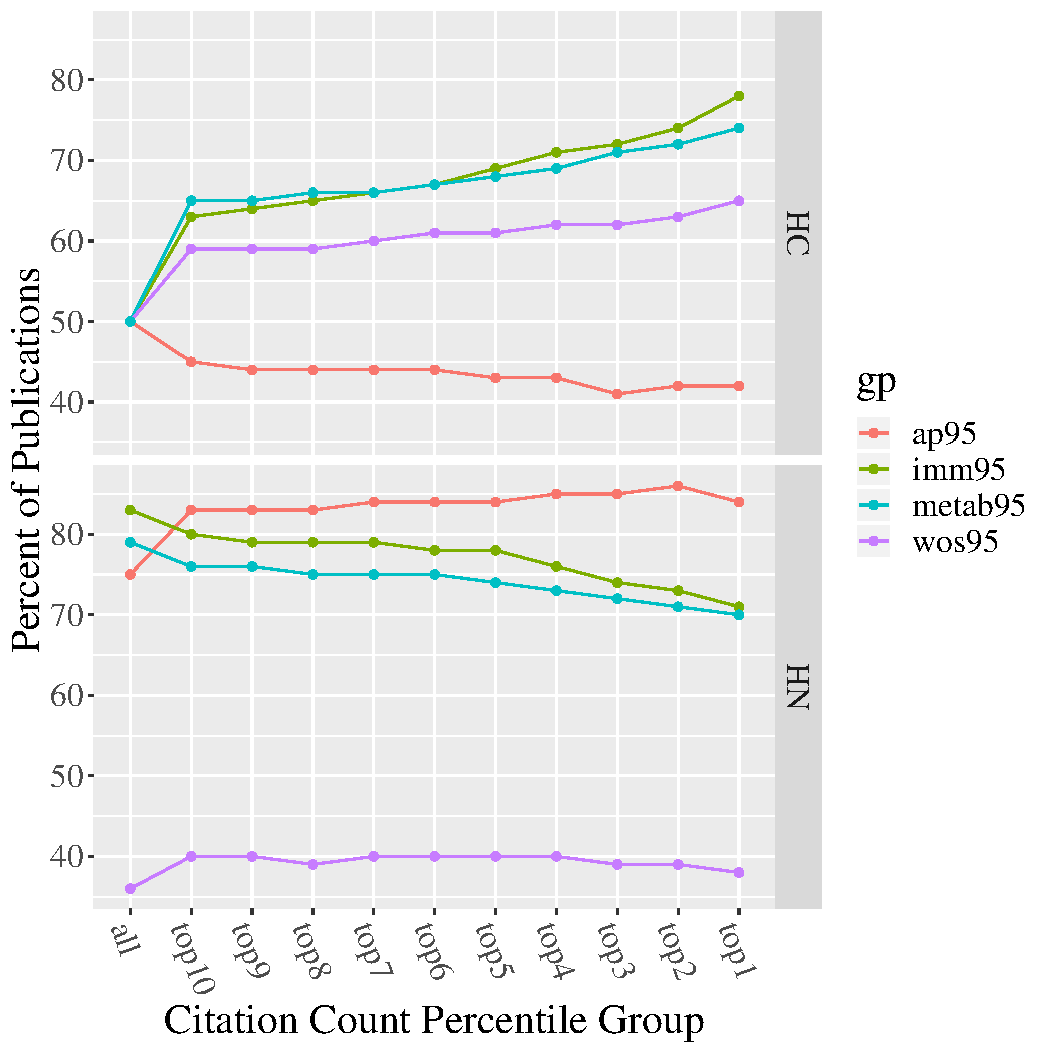
\includegraphics[width=3in]{fig1a.pdf} & 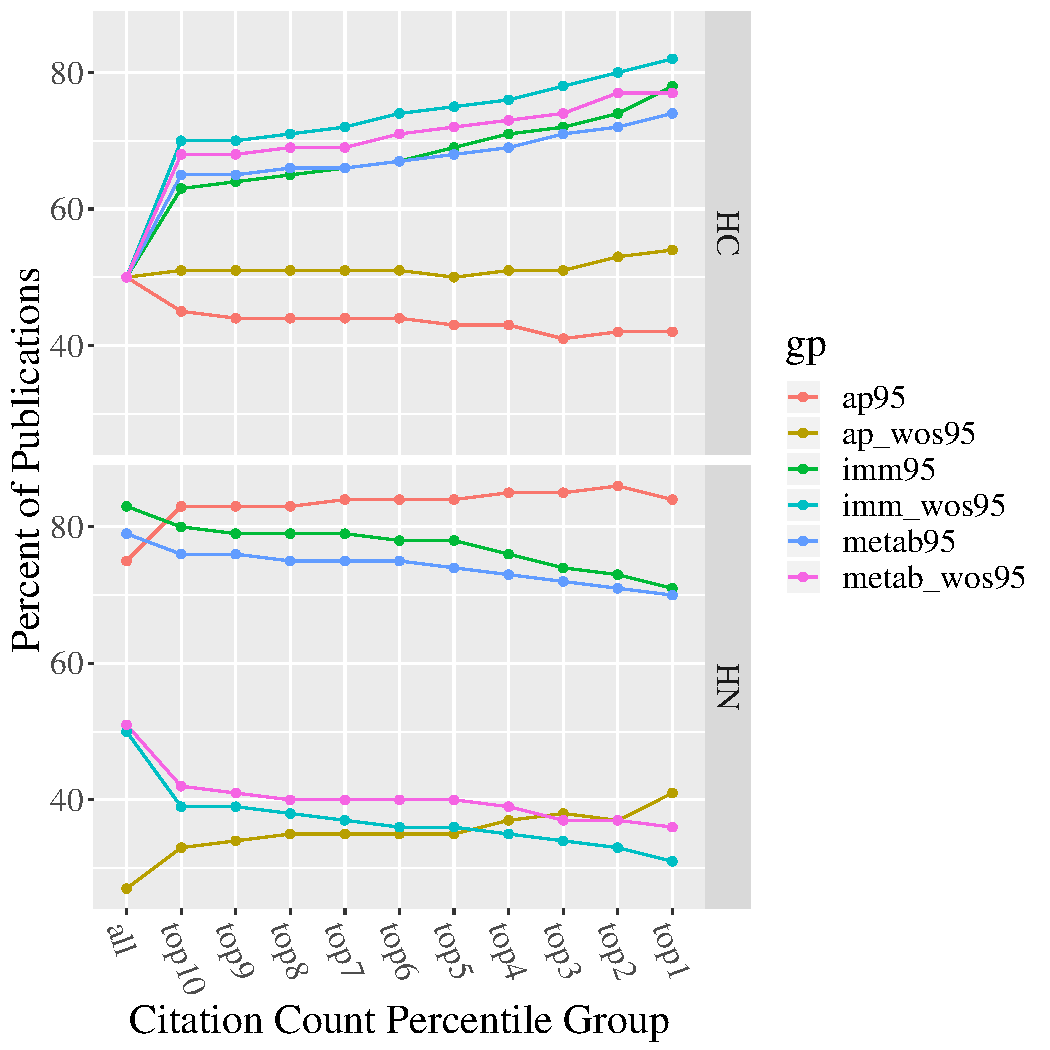
\includegraphics[width=3in]{fig1b.pdf}
\\
(a) & (b)  \\
\end{tabular}
\caption{Effect of Research Discipline,  Background Network,  and Citation Count on Conventionality and Novelty.
Data are shown for the applied physics (18,305), immunology (21,917), metabolism (97,405) and WoS (476,288) networks for 1995; numbers in parentheses are the count of publications in each network.
Subfigures (a) and (b): the x-axis show publications classified into percentile groups based on citation counts (e.g., Top 1 indicates those publications in the top 1\%) and the y-axis shows the percent of publications in each set that are HC or HN.
Based on the selected background network, z-scores are computed for each disciplinary network; thus, \emph{imm} denotes the immunology network with immunology z-scores and \emph{imm\_wos} denotes the immunology network with z-scores from WoS z-scores.
}
\label{fig:Fig1}
\end{figure}
\newpage

 
\emph{On page 2, `In addition, under this random model, a reference cited many times in a given year is selected with the same probability as a reference cited only once, which appears inconsistent with the power law or lognormal citation distributions described in the literature.'  I do not quite understand this.  In Uzzi's reference swapping, for each references, its total number of forward citations is preserved, so at the system level, a reference with fewer citations does have a smaller probability of being swapped.  So I do not exactly understand this criticism.}

Our apologies for not being clear. In the  revised manuscript, we have also highlighted a section of the Materials and Methods that is relevant. In examining the citation shuffling code of Uzzi kindly shared by Satyam Mukherjee and Ben Jones, we realized that the choice of substitutions was restricted to the set rather than the multi-set of eligible references. While their reciprocal substitution approach  ensures that the total number of references stratified by year of publication is still preserved after shuffling, selection of a substituent is equiprobable. In other words, Uzzi's algorithm systematically shuffles every reference but replacements are selected from the set \{a,b,c,d,e\} rather than the multi-set \{aaaa,b,ccc,dd,e\} of eligible references. This flies in the face of what we know about preferential attachment and citation practice. 

Uzzi's citation shuffling code is available on our Github site with permission from the authors. https://bit.ly/2xRsCCM. The key snippet below shows that the references stored in the object below constitute a set, which is selected from during substitution. 

\begin{verbatim}
class Dset(dict):
    def __init__(self, default=None):
        self.default = default

    def __getitem__(self, key):
#        if not self.has_key(key):
        if key not in self:
            self[key] = set()
        return dict.__getitem__(self, key)
\end{verbatim}

In either a local or a global network, it does not make sense to treat a highly cited reference as equiprobable with a reference cited only once. Consider a toy Web of Science dataset consisting of 5 publications all published in the same year. Each of these publications cites 4 references, thus, 20 citations. For simplicity, we will assume that all of these references were published in the same year. Of these, one (which we will call $x$) is cited in each of the publications (thus cited 5 times) and the remaining 15 are cited once in total. During citation shuffling (i)  in our approach, the probability of selecting $x$ would be 5/20 or 1/4. In Uzzi it would be 1/16. The remaining 15 references in Uzzi would have a probability of 1/16, whereas in our model they would have a probability of 1/20. Further, Uzzi's code enforces 20 successive substitution attempts if the original reference is selected as a substitute. Our code allows such a replacement without attempting to artificially enforce substitution with a different reference. Uzzi's code does not check for duplicate references as a result of shuffling, whereas we do and suppress it. The reason we did not emphasize this to a greater extent is because the number of highly cited references is relatively small in a lognormal distribution. Thus, expected values of journal pairs certainly differ between the two algorithmic approaches but our analysis was largely conducted at a high level. Further, the differences between performing 10 (Uzzi) versus 1,000 simulations with better coverage of observed journal pairs (this manuscript) and the effects of the local network seemed more important to focus on. 

The deviation of our results from those of Uzzi et al. can be due to a choice of data set (local vs. global) or sampling technique, and so we compared our sampling approach with Uzzi's to understand how much of the difference was due to the background data set versus the sampling technique. The categorization of articles along the dimension of novelty depends on the sign of z-scores, and so we compared z-scores of each journal-pair with our sampling method versus Uzzi's while keeping  the data set constant.  For the WoS and Applied Physics data sets, we found that 2.8\% and 4.0\% of journal pair z-scores changed sign, respectively.  While this may induce a material effect on whether an article is deemed to be novel, it was apparent that most of the differences in z-scores were due to the background data set and so we did not comment further in the submission on the differences in sampling techniques.


\end{document}  